\section{¡Triángulos!... ¿Otra vez?}

El día de hoy trabajaremos con el \textit{Triangulo de Pascal}. Si no lo conoces, te lo presento:

\begin{center}
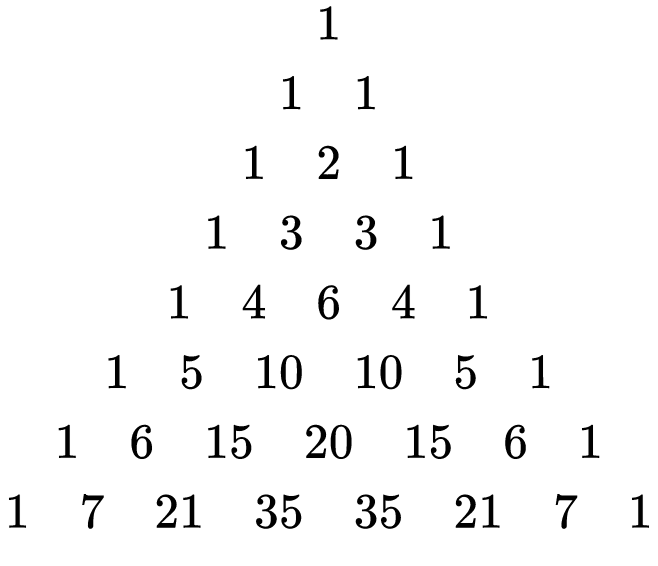
\includegraphics[scale=0.5]{Imagenes/pascal}

\textit{Robadisimo} desde Wikipedia\texttrademark\footnote{https://en.wikipedia.org/wiki/Pascal\%27s\_triangle}
\end{center}

El funcionamiento de este árbol es el siguiente:
\begin{itemize}
    \item La primera fila tiene un único numero, el número 1.
    \item La segunda fila contiene 2 números, ambos 1.
    \item Las siguientes filas contienen el numero 1 en los extremos, y cada numero se compone de la suma de los 2 números que están justo encima de ese numero.
\end{itemize}

Ahora que ya sabes como puede ser construida la pirámide de Pascal, te invito a que escribas la función \texttt{piramide\_de\_pascal(n)}, la cual recibe un número \texttt{n} mayor o igual a 1, y retorna una lista de listas, la cual contiene la pirámide de Pascal. Esta pirámide tiene las primeras \texttt{n} filas de la pirámide de Pascal.

\begin{lstlisting}[style=consola]
>>> [*pascal = piramide_de_pascal(6)*]
>>> [*for i in pascal:*]
>>> [*    print(i)*]
[1]
[1, 1]
[1, 2, 1]
[1, 3, 3, 1]
[1, 4, 6, 4, 1]
[1, 5, 10, 10, 5, 1]
\end{lstlisting}

